\documentclass[a4paper,oneside,12pt]{extreport}

\usepackage{mmap}
\usepackage[T2A]{fontenc}
\usepackage[utf8]{inputenc}
\usepackage[english,russian]{babel}


% Текст отчёта следует печатать, соблюдая следующие размеры полей:
% левое — 30 мм, правое — 15 мм, верхнее и нижнее — 20 мм.
\usepackage[left=20mm, right=15mm, top=15mm, bottom=15mm]{geometry}

% \setlength{\parindent}{1.25cm} % Абзацный отступ

\usepackage{setspace}
%\onehalfspacing % Полуторный интервал

\frenchspacing % Равномерные пробелы
\usepackage{indentfirst} % Красная строка

\usepackage{microtype}
\sloppy

\usepackage{titlesec}
\titlespacing*{\chapter}{0pt}{-30pt}{8pt}
\titlespacing*{\section}{\parindent}{*4}{*4}
\titlespacing*{\subsection}{\parindent}{*4}{*4}
\titleformat{\chapter}{\LARGE\bfseries}{\thechapter}{20pt}{\LARGE\bfseries}
\titleformat{\section}{\Large\bfseries}{\thesection}{40pt}{\Large\bfseries}

\usepackage{graphicx}
\usepackage{caption}

\usepackage[unicode,pdftex]{hyperref}
\hypersetup{hidelinks}

%% title begin
\usepackage{wrapfig}

\makeatletter
	\def\vhrulefill#1{\leavevmode\leaders\hrule\@height#1\hfill \kern\z@}
\makeatother
%% title end

%% begin code
\usepackage{listings}
\usepackage{xcolor}

\lstset{
	basicstyle=\footnotesize\ttfamily,
	breakatwhitespace=true,
	breaklines=true,
	commentstyle=\color{gray},
	frame=single,
	keywordstyle=\color{blue},
	stringstyle=\color{red},
	tabsize=8
}

\lstdefinestyle{lispinline}{
	frame=none,
	language=Lisp
}

\newcommand{\code}[1]{\texttt{#1}}
%% end code

%% begin theorem
\usepackage{amsthm}

\makeatletter
\newtheoremstyle{indented}
	{}% measure of space to leave above the theorem
	{}% measure of space to leave below the theorem
	{}% name of font to use in the body of the theorem
	{\parindent}% measure of space to indent
	{\bfseries}% name of head font
	{.}% punctuation between head and body
	{ }% space after theorem head; " " = normal interword space
	{}% header specification (empty for default)
\makeatother

\theoremstyle{indented}

\newtheorem{definition}{Определение}[section]
\newtheorem{example}{Пример}[section]
\newtheorem{theorem}{Теорема}[section]
\newtheorem{task}{Задание}

\makeatletter
\DeclareRobustCommand\bfseriesitshape{%
	\not@math@alphabet\itshapebfseries\relax
	\fontseries\bfdefault
	\fontshape\itdefault
	\selectfont
}
\makeatother

\DeclareTextFontCommand{\textbfit}{\bfseriesitshape}
\DeclareTextFontCommand{\define}{\bfseriesitshape}
%% end theorem

%% begin columns
\usepackage{etoolbox,refcount}
\usepackage{multicol}

\newcounter{countitems}
\newcounter{nextitemizecount}
\newcommand{\setupcountitems}{%
	\stepcounter{nextitemizecount}%
	\setcounter{countitems}{0}%
	\preto\item{\stepcounter{countitems}}%
}
\makeatletter
\newcommand{\computecountitems}{%
	\edef\@currentlabel{\number\c@countitems}%
	\label{countitems@\number\numexpr\value{nextitemizecount}-1\relax}%
}
\newcommand{\nextitemizecount}{%
	\getrefnumber{countitems@\number\c@nextitemizecount}%
}
\newcommand{\previtemizecount}{%
	\getrefnumber{countitems@\number\numexpr\value{nextitemizecount}-1\relax}%
}
\makeatother
\newenvironment{AutoMultiColItemize}{%
	\ifnumcomp{\nextitemizecount}{>}{3}{\begin{multicols}{2}}{}%
		\setupcountitems\begin{itemize}}%
		{\end{itemize}%
		\unskip\computecountitems\ifnumcomp{\previtemizecount}{>}{3}{\end{multicols}}{}}
\makeatother
\newenvironment{AutoMultiColEnumerate}{%
	\ifnumcomp{\nextitemizecount}{>}{3}{\begin{multicols}{2}}{}%
		\setupcountitems\begin{enumerate}}%
		{\end{enumerate}%
		\unskip\computecountitems\ifnumcomp{\previtemizecount}{>}{3}{\end{multicols}}{}}
%% end columns



\begin{document}

\begin{titlepage}
	{\large % 14pt instead of 12pt
	\onehalfspacing
	\centering

	\begin{wrapfigure}[7]{l}{0.14\linewidth}
		\vspace{3mm}
		\hspace{-10mm}
		
\includegraphics[width=\linewidth]{img/b_logo}
		% \includegraphics[width=0.93\linewidth]{inc/img/bmstu-logo}
	\end{wrapfigure}
	{\singlespacing \footnotesize \bfseries Министерство науки и высшего образования Российской Федерации\\Федеральное государственное бюджетное образовательное учреждение\\высшего образования\\<<Московский государственный технический университет\\имени Н.~Э.~Баумана\\ (национальный исследовательский университет)>>\\(МГТУ им. Н.~Э.~Баумана)\\}

	\vspace{-2.2mm}
	\vhrulefill{0.9mm}\\
	\vspace{-7.5mm}
	\vhrulefill{0.2mm}\\
	\vspace{2mm}

	{\doublespacing \small \raggedright ФАКУЛЬТЕТ \hspace{5mm} \underline{«Информатика и системы управления»}\\
	КАФЕДРА \hspace{10mm} \underline{«Программное обеспечение ЭВМ и информационные технологии»}\\}

	\vspace{20mm}

	\begin{center}
		\noindent\begin{minipage}{1.2\textwidth}\centering
			\textbf{ОТЧЕТ ПО ЛАБОРАТОРНОЙ РАБОТЕ №18,19}\newline
			\textbf{По курсу: "Функциональное и Логическое программирование"}\newline\newline\newline
		\end{minipage}
	\end{center}

	\vspace{20mm}

	\noindent ~~Тема \underline{~~~~~~~~~~~~~~~~~~~~~~~~~~Рекурсия в прологе.~~~~~~~~~~~~~~~~~~~~~~~~~~~~~~~~~~~~~~~~~~~}\newline
	\noindent ~~Группа \underline{~~~~~~~~~~~~~~~~~~~~~~~~~~~~~~~~~~~ИУ7-63Б~~~~~~~~~~~~~~~~~~~~~~~~~~~~~~~~~~~~~~~~~~~~~~~~~}\newline
	\noindent ~~Студент \underline{~~~~~~~~~~~~~~~~~~~~~~~~~~~~Сукочева А.~~~~~~~~~~~~~~~~~~~~~~~~~~~~~~~~~~~~~~~~~~~~~~~~~~}\newline
	\noindent ~~Преподаватель \underline{~~~~~~~~~~~~~~~~~Толпинская Н.Б.~~~~~~~~~~~~~~~~~~~~~~~~~~~~~~~~~~~~~~~~~~~~~}\newline
	\noindent ~~Преподаватель \underline{~~~~~~~~~~~~~~~~~~Строганов Ю. В.~~~~~~~~~~~~~~~~~~~~~~~~~~~~~~~~~~~~~~~~~~~~}\newline


	\begin{center}
		\vfill
		Москва~---~\the\year
		~г.
	\end{center}
	}



\end{titlepage}

\setcounter{page}{2}

\section*{Теоретическая часть}

\subsection*{Логическое программирование}

\textbf{Логическое программирование} -- это программирование на знаниях. 
Логическое программирование принципиально работает не с данными, а со знаниями.
% В отличии от императивных яп (в них определяется порядком записи правил (команд) 
Порядок действий в системе логического программирования prolog определяется алгоритмом унификации. 

Программируя на императивным я.п., программист должен задать порядок действий,
(который в дальнейшем будет последовательно выполнен), т.е. объяснить компьютеру \textbf{как} решать задачу.
В случае декларативного я.п. программист должен описать \textbf{что} нужно решить (А уже с помощью алгоритма унификации будет решена задача)

\subsection*{Элементы языка}

\textbf{Элементы языка}: терм.

\textbf{Терм} - это:
\begin{enumerate}
    \item \textbf{константа}:
    \begin{enumerate}
        \item число (пример: 1; 55; 12.32);
        \item символьный атом. Начинается со  \textbf{строчной} буквы и используется для обозначения конкретного объекта предметной области или для обозначения конкретного отношения (пример: alice, iu7\_63B);
        \item строка - последовательность символов, заключенная в кавычки (пример: "Элис Сукочева").
    \end{enumerate}
    \item \textbf{переменная}
    \begin{enumerate}
        \item Именнованная - комбинация символов, цифр и '\_', которая начинается с \textbf{прописной} буквы или с символа '\_' (пример: Name, \_A). Переменные могут связываться с различными объектами – конкретизироваться;
        \item Анонимная - обозначается символом '\_'. Анонимные переменные не могут быть связаны со значением.
    \end{enumerate}
    \item \textbf{составной терм} - взаимосвязанная информация. Показывает связь между объектами. Т.е. кто от чего зависит. 
    Синтаксис: \textbf{$f(t_1, t_2, ... , t_m)$}, где $f$ - функтор - символьная константа, обозначающая имя отношения. $t_1$, $t_2$, ... , $t_m$ - термы, являющиеся аргументами. Арность - число аргументов. (Пример: учится(элис, мгту) - знание о то, что Элис учится в МГТУ.
\end{enumerate}


\subsection*{Программа на prolog}

\textbf{Программа на prolog} - база знаний и вопрос. 

База знаний - это факты и правила. Каждое предложение (факт или правило) должно заканчиваться точкой.

\textbf{Правило} имеет вид:
    A :- $B_1$, ... , $B_n$
    
A - заголовок правила (терм).

$B_1$, ... , $B_n$ - тело правила (термы). 

Символ ":-" это специальный символ-разделитель.

\textbf{Факт} – это частный случай правила. Факт – это предложение, в котором отсутствует тело
(т.е. тело пустое). 
% В фактах присутствую только заголовки, а значит знания в заголовках.

\textbf{Заголовок} - составной терм, который содержит знание. Знания в заголовках.

\textbf{В теле} прописаны условия истинности этого знания (которое написано в заголовке).

В разделе \textbf{CLAUSES} записываются факты и правила.

Пример:

\begin{lstlisting}[language=Prolog]
CLAUSES
    study(alice, bmstu).
    study(ivan, bmstu).
\end{lstlisting}
    
% Вопрос - вид предложения.
\textbf{Вопрос} - частный случай правила, состоит только из тела (составного терма или нескольких составных термов).
Используется, чтобы определить, выполняется ли некоторое отношение между описанными в программе объектами.
Ответом может быть "Yes" или "No".

В разделе GOAL содержатся цели, которые нужно достигнуть. 
Главная задача заключается в том, чтобы дать ответ "Yes" на поставленный вопрос.
В случае, если система не может ответить "Yes", система отвечает "No".

Пример:
\begin{lstlisting}[language=Prolog]
GOAL
    study(alice, bmstu) % Yes
\end{lstlisting}

% Переменные предназначены для передачи значений "во времени и в пространстве".
% Конкретизация переменной - связь переменной с объектом.

\subsection*{Механизм унификации}
\textbf{Механизм унификации} (подбор нужного решения).
Поиск ответа на поставленный вопрос заключается в поиске нужного знания с помощью механизма унификации. Данный механизм встроен в систему и недоступен программисту.

\textbf{Процедуры} - совокупность правил, заголовки которых имеют одно и то же имя и одну и ту же арность.

\textbf{Предикат} - отношение, определяемое процедурой.

\section*{Практическая часть л.р.1}

\begin{task}
    Разработать свою программу - «Телефонный справочник».
    Протестировать работу программы.
    \begin{lstlisting}[language=Prolog]
PREDICATES
	phonebook(phone, name, school\_number).

CLAUSES 
	phonebook("+79998881234", "Alice", 433).
	phonebook("+79998881235", "Pasha", 415).
	phonebook("+79998881236", "Nastya", 433).
	phonebook("+79998881237", "Ivan", 424).
	phonebook("+79998881238", "Dima", 123).
	phonebook("+79998881134", "Oleg", 123).
	phonebook("+79991881334", "Nikita", 25).
	phonebook("+79998391234", "Misha", 1024).

GOAL
	phonebook(Phone_number, Name, 433).
    \end{lstlisting}
\end{task}

\section*{Практическая часть л.р.2}

\begin{task}
    Составить программу – базу знаний, с помощью которой можно определить, например, 
    множество студентов, обучающихся в одном ВУЗе. 
    Студент может одновременно обучаться в нескольких ВУЗах. 
    Привести примеры возможных вариантов вопросов и варианты ответов
    (не менее 3-х).

    \begin{lstlisting}[language=Prolog]
DOMAINS 
    student_id = integer.
    student_name = symbol.
    student_surname = symbol.
    
    university_id = integer.
    university_name = symbol.
    city = symbol.

PREDICATES
    study(student_id, university_id).
    student(student_id, student_name, student_surname).
    university(university_id, university_name, city).
    
    students(university_id, student_name, student_surname).
    
CLAUSES
    student(0, "Alice", "Sukocheva").
    student(1, "Nika", "Lilova").
    student(2, "Masha", "Perestoronina").
    student(3, "Pasha", "Perestoronin").
    student(4, "Nastya", "Namestnik").
    student(5, "Kirill", "Drovin").
    student(6, "Tim", "Malov").
    
    university(0, "Bauman Moscow State Technical University", "Moscow").
    university(1, "Petersburg State University", "Petersburg").
    university(2, "Kuban State University", "Krasnodar").
    
    study(0, 0).
    study(2, 0).
    study(3, 0).
    study(4, 0).
    
    study(5, 2).
    study(5, 0).
    
    study(6, 0).
    study(6, 1).
    study(6, 2).
    
    students(University_id, Name, Surname) :- 
            study(Student_id, University_id), 
            student(Student_id, Name, Surname).
    
GOAL
    % All infomation about students. 
    % student(Id, Name, Surname).
    
    % All infomation about universities.
    % university(Id, Name, City).
    
    % All id students from the university.
    % study(Id, 0). % 0, 2, 3, 4, 5, 6
    % study(Id, 1). % 6
    % study(Id, 2). % 5, 6

    % All name and surname students from the university.
    % students(0, Name, Surname).
    % students(1, Name, Surname).
    % students(2, Name, Surname).
    
    % All universities where the student studies.
    % study(0, U_id). % 0
    % study(1, U_id). % study(0, U_id). 
    study(6, U_id). % 0, 1, 2
    \end{lstlisting}

    На рис. \ref{ref:fig1} продемонстрировано определение id вузов, 
    в которых учится студент с id = 6.

    \begin{figure}[ht!]
    	\centering{
    		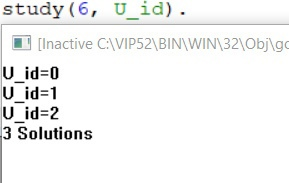
\includegraphics[width=0.5\textwidth]{img/1.jpg}
    		\caption{Результат работы 1.} 
            \label{ref:fig1}}
    \end{figure}

    На рис. \ref{ref:fig2} продемонстрировано определение имени и фамилии студентов,
    обучающихся в вузе с id равным двум. 


    \begin{figure}[ht!]
    	\centering{
    		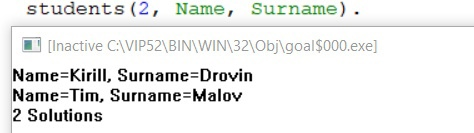
\includegraphics[width=0.7\textwidth]{img/2.jpg}
    		\caption{Результат работы 2.} 
            \label{ref:fig2}}
    \end{figure}

    На рис. \ref{ref:fig3} продемонстрировано определение имени и фамилии студентов,
    обучающихся в вузе с id равным 0. 


    \begin{figure}[ht!]
    	\centering{
    		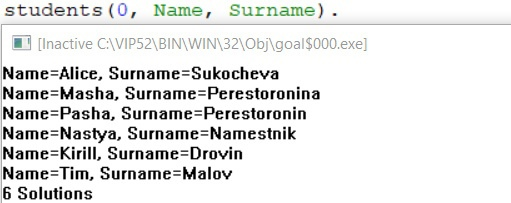
\includegraphics[width=0.65\textwidth]{img/3.jpg}
    		\caption{Результат работы 3.} 
            \label{ref:fig3}}
    \end{figure}

    На рис. \ref{ref:fig4} продемонстрировано определение id студентов,
    обучающихся в вузе с id равным 0.

    \begin{figure}[ht!]
    	\centering{
    		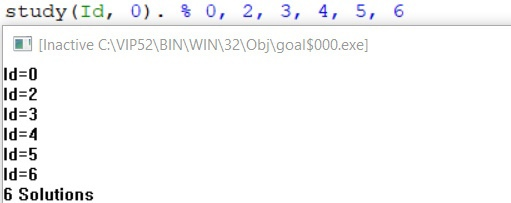
\includegraphics[width=0.65\textwidth]{img/4.jpg}
    		\caption{Результат работы 4.} 
            \label{ref:fig4}}
    \end{figure}

    На рис. \ref{ref:fig4} продемонстрировано определение 
    всех имеющихся в базе данных вузов.     

    \begin{figure}[ht!]
    	\centering{
    		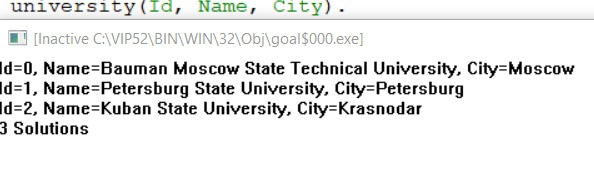
\includegraphics[width=0.65\textwidth]{img/5.jpg}
    		\caption{Результат работы 5.}
            \label{ref:fig5} }
    \end{figure}

\end{task}

\section*{Практическая часть л.р.3}

\begin{task}
    Составить программу, т.е. модель предметной области – базу знаний, объединив в ней
    информацию – знания:
    \begin{enumerate}
        \item Телефонный справочник: Фамилия, Номер телефона, Адрес – структура (Город, Улица, Noдома, Noкв),
        \item Автомобили: Фамилия владельца, Марка, Цвет, Стоимость, и др.,
        \item Вкладчики банков: Фамилия, Банк, счет, сумма, др.
    Владелец может иметь несколько телефонов, автомобилей, вкладов (Факты).
    Используя правила, обеспечить возможность поиска:
    \end{enumerate}

    1. а) По номеру телефона найти: Фамилию, Марку автомобиля, Стоимость автомобиля
    (может быть несколько),
    в) Используя сформированное в пункте а) правило, по номеру телефона найти:
    только Марку автомобиля (автомобилей может быть несколько),
    
    2. Используя простой, не составной вопрос: по Фамилии (уникальна в городе, но в
    разных городах есть однофамильцы) и Городу проживания найти:
    Улицу
    проживания, Банки, в которых есть вклады и номер телефона.

    \begin{lstlisting}[language=Prolog]
DOMAINS 
	surname = symbol.
	phone_number = symbol.
	address_struct = address(symbol, symbol, integer, integer).

	label = symbol.
	color = symbol.
	price = integer.
	
	bank = symbol.
	score = integer.
	sum = integer.

PREDICATES
	phonebook(surname, phone_number, address_struct).
	car(surname, label, color, price).
	bank_depositor(surname, bank, score, sum).
	
	f1(surname, phone_number, label, price).
	f1_2(phone_number, label).
	f2(surname, symbol, phone_number, symbol, bank).

CLAUSES
	phonebook("Tilov", "89999899999", address("Moscow", "2 baumanskaya", 57, 25)).
	phonebook("Tilov", "89999899977", address("Moscow", "2 baumanskaya", 57, 25)).
	phonebook("Alovik", "89999812999", address("Moscow", "3 baumanskaya", 50, 75)).
	
	car("Tilov", "Buick", "black", 12000000).
	car("Tilov", "Cadillac", "white", 22000000).
	
	bank_depositor("Alovik", "sberbank", 10000, 25000).
	bank_depositor("Alovik", "vtb", 20000, 35000).
	
	f1(Surname, Phone_number, Label, Price) :-  
		phonebook(Surname, Phone_number, _), 
		car(Surname, Label, _, Price). 
		
	f1_2(Phone_number, Label) :- 
		f1(_, Phone_number, Label, _).
	
	f2(Surname, City, Phone_number, Street, Bank) :- 
		phonebook(Surname, Phone_number, address(City, Street, _, _)), bank_depositor(Surname, Bank, _, _).
	
GOAL
	f1(Surname, "89999899999", Label, Price).
	% f1_2("89999899999", Label).
	% f2("Alovik", "Moscow", Phone_number, Street, Bank).
    \end{lstlisting}

\end{task}

\newpage

\section*{Ответы на вопросы}

1. Что собой представляет программа на Prolog

Программа на Prolog представляет базу знаний и вопрос.

2. Какова ее структура. 

Структура программы на Prolog.

\begin{enumerate}
    \item директивы компилятора — зарезервированные символьные константы. (Пример ":-" - разделитель между заголовком и телом в правиле) 
    \item CONSTANTS — раздел описания констант.
    \item DOMAINS — раздел описания доменов.
    \item DATABASE — раздел описания предикатов внутренней базы данных.
    \item PREDICATES — раздел описания предикатов.
    \item CLAUSES — раздел описания предложений базы знаний.
    \item GOAL — раздел описания внутренней цели (вопроса).
\end{enumerate}

3. Как она реализуется.

Описывается база знаний и задается вопрос.

4. Как формируются результаты работы программы. 

Система пытается найти такие значения переменных, при которых можно ответить на поставленный вопрос 'Да', используя базу знаний. %, путем унификации.


\end{document}